\section{Red laboral}
Para explorar nuevas topologias y relaciones decidimos monitorear una red laboral en una oficina de mediana envergadura. En esta
red local conviven nodos de empleados, servidores de distinto uso, asi como impresoras de red y otros dispositivos de oficina. 

El primer experimento, el cual ve la red como una fuente con 2 simbolos unicamente, monitoreo la red local a traves de un enlace
ethernet durante 20 minutos. Como era de esperarse cerca del 100\% del trafico es unicast dado que es una red con mucho trafico
hacia un servidor en particular o hacia el gateway.

\begin{figure}[!h]
\centering
\caption{Informaci'on de S, Red laboral}
\begin{tabular}{ r|c|c| }
\multicolumn{1}{r}{}
 &  \multicolumn{1}{c}{frecuencia}
 & \multicolumn{1}{c}{informaci'on} \\
\cline{2-3}
$S_{broadcast}$ & 0.03 & 5.06 \\
\cline{2-3}
$S_{unicast}$ & 0.97 & 0.04 \\
\cline{2-3}
\end{tabular}
\end{figure}
 
 Estos valores nos dan una entrop'ia de 0.19 bits (siendo el m'aximo 1 dado que hay 2 simbolos en principio equiprobables),
 dado que el trafico broadcast sin ser despreciable solo es un porcentaje peque\~no del trafico total.\\
 
En el segundo experimento, el cual modela la red basado en la direcci'on a resolver en mensajes ARP, usamos la misma captura
utilizada en el experimento anterior. Bajo nuestra definici'on para destacar nodos (que la informaci'on del simbolo de ese nodo 
sea menor o igual a la entrop'ia de la fuente) solo un nodo fue destacado por amplio margen, el gateway por defecto de la red.\\

\begin{figure}[!h]
\centering
\caption{Informaci'on red laboral}
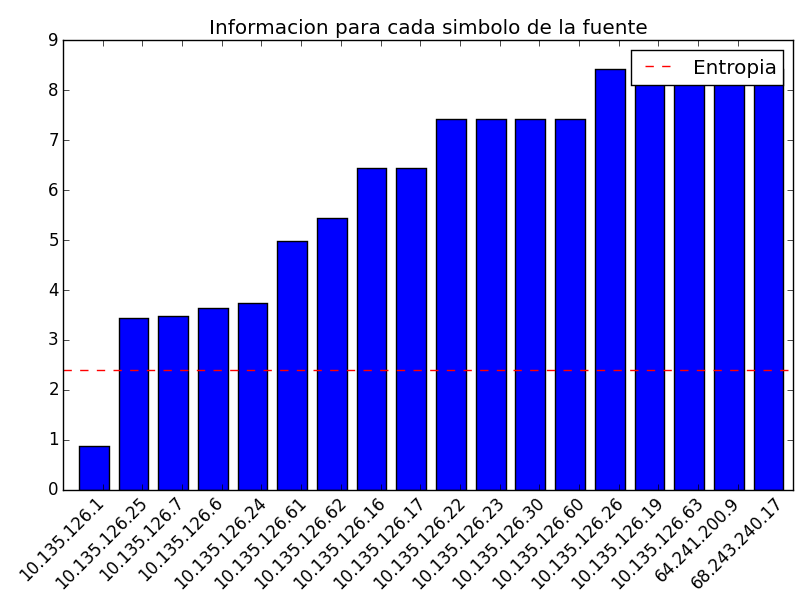
\includegraphics[width=0.55\textwidth]{red2_info}
 \label{fig:red2info}
\end{figure}

La visualizaci'on de la red modelada como la fuente descriptiva muestra una topologia y relaci'on entre nodos muy similar
a la realidad en terminos de trafico total y disposici'on.

\begin{figure}[!h]
\centering
\caption{Visualizaci'on red laboral, en amarillo los nodos destacados}
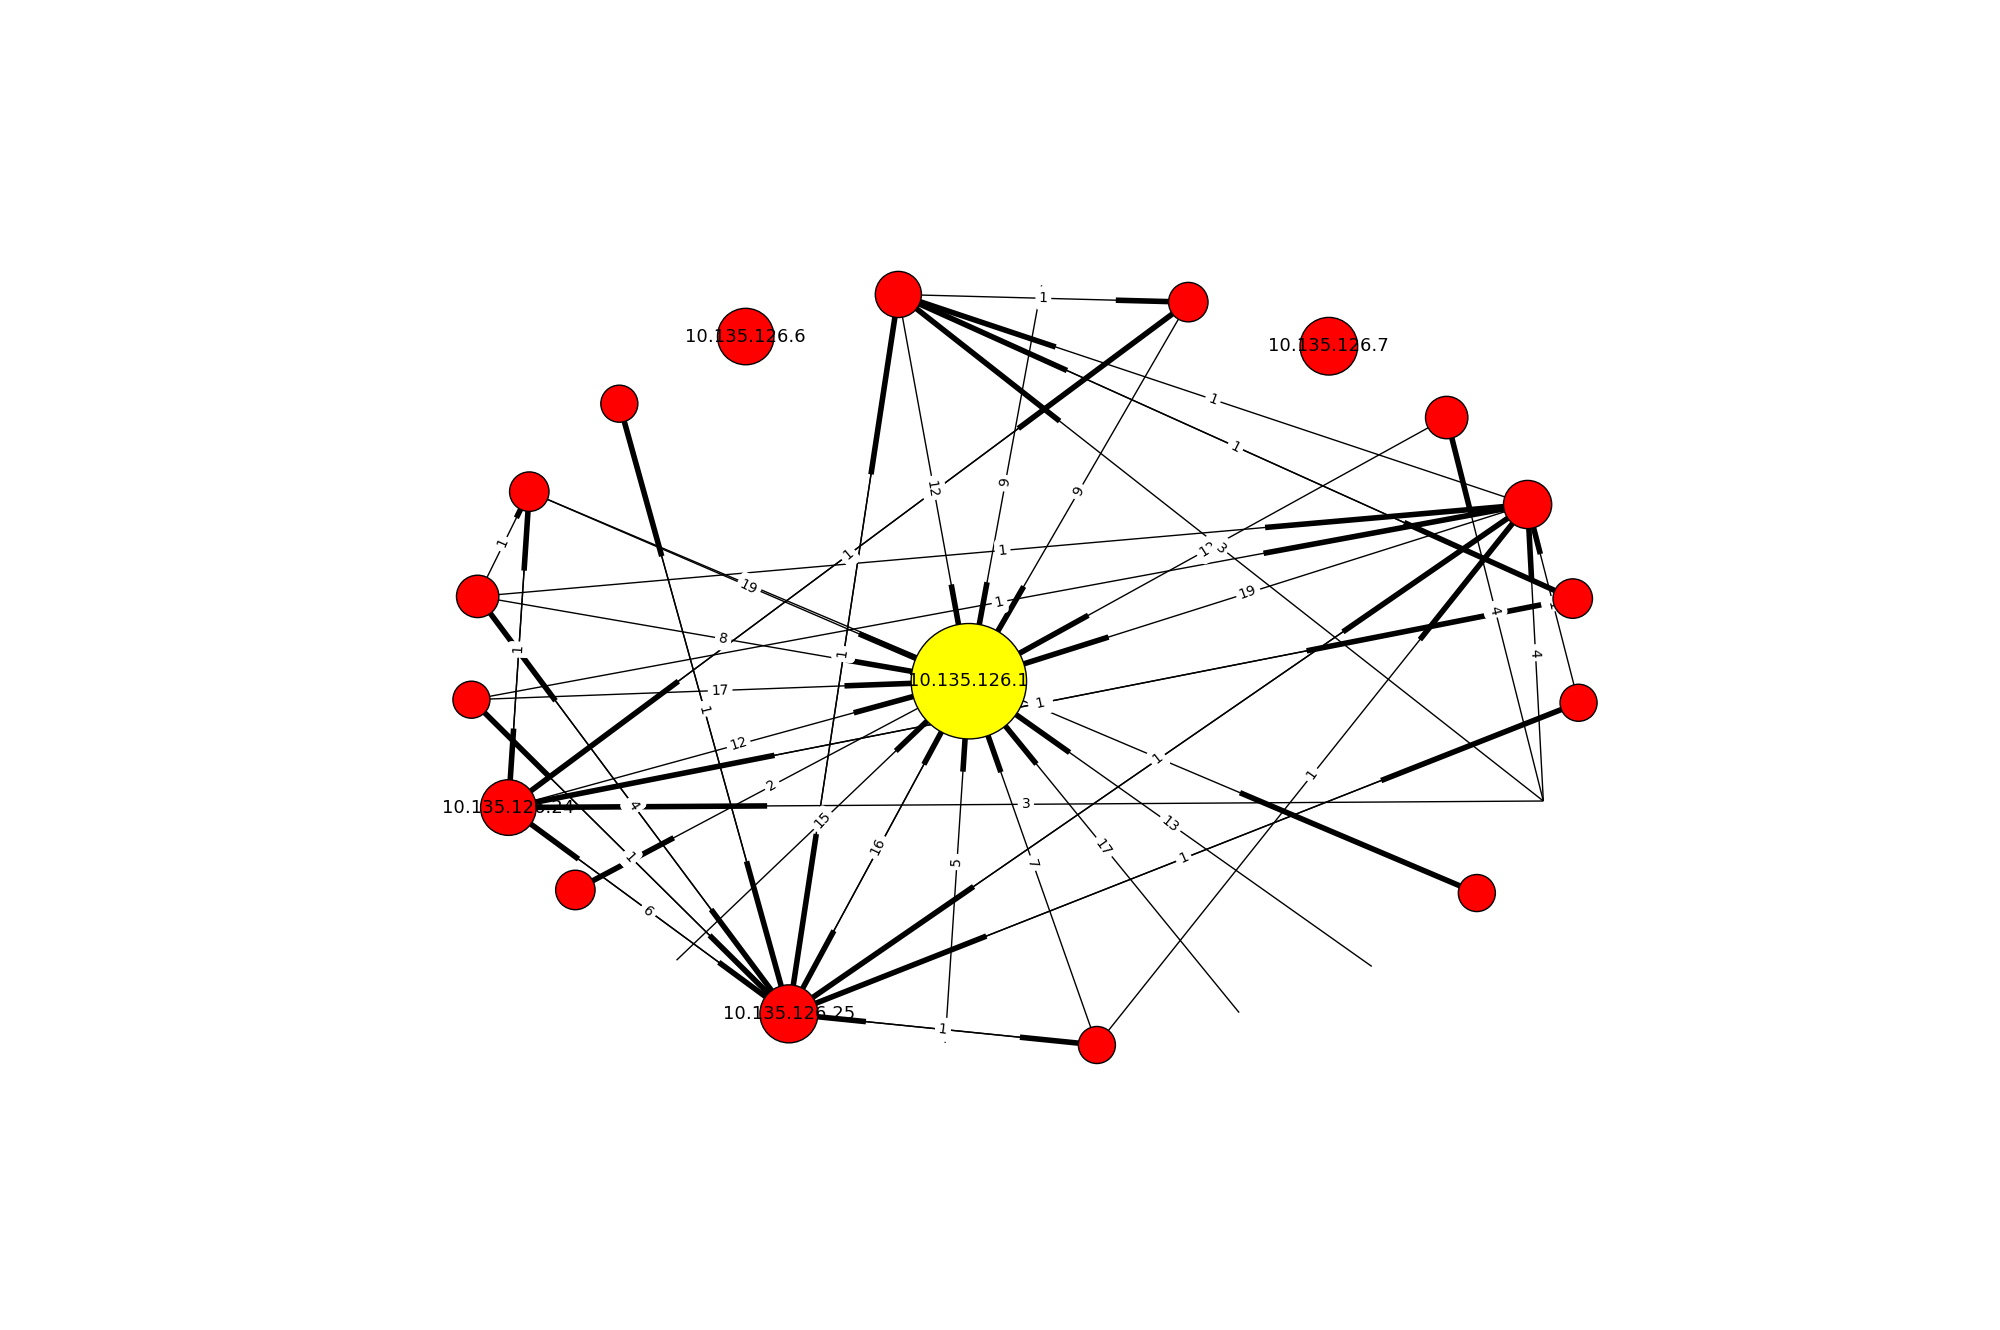
\includegraphics[width=0.9\textwidth]{red2_red}
 \label{fig:red2net}
\end{figure}

Un analisis manual del trafico mostr'o 2 fenomenos de ARP no usuales, ARP gratuitos y ARP de sondeo. Los ARP gratituitos pueden
ser tanto \texttt{who-has} como \texttt{is-at} donde la direcci'on de origen como destino son las mismas (y la direcci'on
de enlace destino es broadcast). El uso de los mismos es precargar o refrescar las tablas de otros nodos para evitar tener
que traducir en tiempo real una direcci'on de red. Los ARP de sondeo tienen un fin similar, un nodo al que se le asigno manualmente
o automaticamente una direcci'on de red, envia un ARP con dicha direcci'on a la red y si alg'un nodo le responde entonces sabra
que la direcci'on ya esta en uso y evitara la colisi'on de alguna forma. Ning'un de estos tipos de mensajes estan oficialmente
documentados pero forman parte de toda red que necesite autoregularse correctamente.\\
